\chapter{Biblioteczka zastępowego}
\begin{wrapfigure}{l}{4cm}
  \begin{center}
    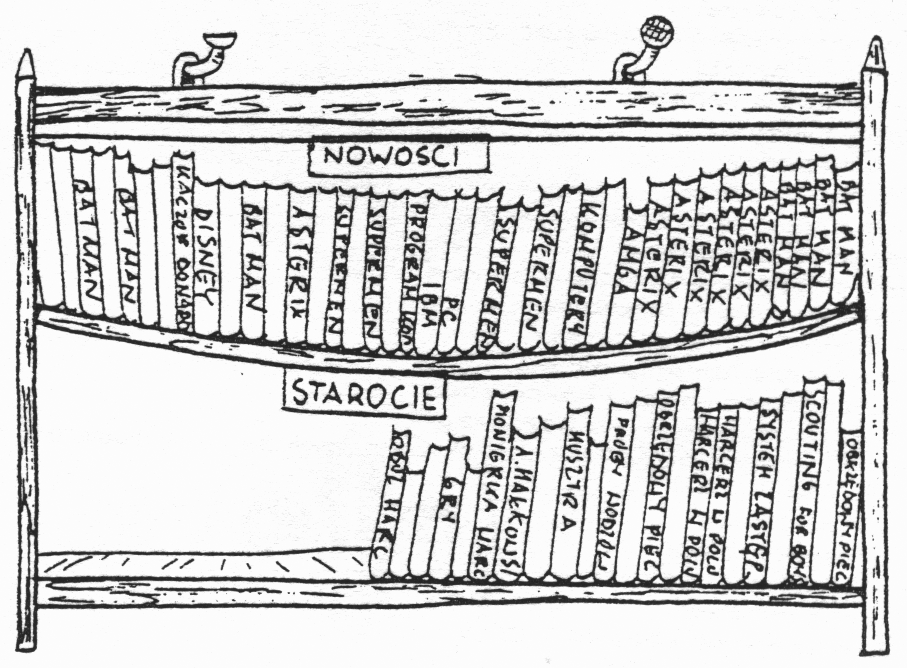
\includegraphics[width=4cm]{grafiki/biblioteczka.png}
  \end{center}
\end{wrapfigure} Spis ten nie wyczerpuje wszystkich pozycji przydatnych zastępowemu, do tej listy dołączyć należałoby wiele innych książek o tematyce historycznej, przygodowej, krajoznawczej. W biblioteczce zastępowego powinno być miejsce także dla śpiewników, map, czasopism, wydawnictw okazjonalnych itp. Biblioteka zastępowego to kopalnia pomysłów na zbiórki, wyprawy... Pamiętajcie jednak by nie zżynać dokładnie z książek, twórzcie w oparciu o to co przeczytaliście nowe, lepsze, ciekawsze formy pracy!
\begin{multicols}{2}
\begin{itemize}[noitemsep,nolistsep] 
\small
\item	R. Baden-Powell - Skauting dla chłopców
\item	R. Baden-Powell – Wskazówki dla skautmistrzów
\item	W. Błażejewski - Z dziejów harcerstwa polskiego
\item	A. Chmielewski - Tropy i ślady zwierząt
\item	M. Cmielowa - Wykapka
\item	J. Dąbrowski - Gry i zabawy w izbie harcerskiej
\item	J. Dąbrowski - Harce zimowe
\item	J. Dąbrowski - W świetlicy harcerskiej
\item	J. Dąbrowski i T. Kwiatkowski - Jeden trudny rok
\item	A. Dziewanowska, K. Rejs i Z. Zakrzewska - Gry i ćwiczenia w zastępie harcerskim
\item	S. Gawkowski - Szkice polowe harcerza
\item	E. Grodecka i J. Zwolakowska - Ćwiczenia i gry
\item	A. Gromski - Harce młodzika i wywiadowcy
\item	W. Hansen – Wilk, który nigdy nie śpi
\item	J. Jasiński - Gry i ćwiczenia terenowe
\item	A. Kamiński - A. Małkowski
\item	A. Kamiński - Kamienie na szaniec
\item	A. Kamiński - Zośka i Parasol
\item	M. Kapiszewska - Księga Harców R.Philips - System zastępowy
\item	A. Kazanecki - Terenoznawstwo dla harcerzy
\item	A. Kazanecki - Z notatnikiem i busolą - zbiór gier
\item	B. Kowalska i A. Kiewicz - Eskimos (materiały do zbiórek)
\item	M. Kudasiewicz - Obrzędowy piec
\item	T. Kwiatkowski - Obrzędy harcerskie
\item	O. Małkowska - A. Małkowski
\item	O. Nassalski - Jak pracować nad charakterem
\item	W. Nekrasz - Pionierka harcerska
\item	J. Parzyński - Obóz harcerski
\item	A. Pawełek - Młoda drużyna
\item	W. Pijanowski - Rozkosze łamania głowy
\item	W. Pijanowski - Skarbnica gier
\item	St. Sedlaczek - Drogowskaz Harcerza
\item	St. Sedlaczek - Geneza skautingu i harcerstwa
\item	St. Słysz - Gry i zabawy
\item	St. Sosnowski i J. Stykowski - Sakwa włóczykija
\item	W. Śliwerski - Harcerskie biegi
\item	J. Stykowski - Na traperskiej ścieżce
\item	J. Stykowski - Wyspa Robinsona
\item	J. Stykowski - Zastęp zbiórka (cykl 4 częściowy: wiosna, lato, jesień, zima)
\item	W. Szczygieł - Jak prowadzić zastęp harcerski
\item	W. Szyrzyński - Ambulans harcerski
\item	W. Szyrzyński - Wycieczki harcerskie
\item	Z. Trylski - Mały podręcznik obozowania
\item	Z. Trylski - Obozy 
\item	L. Ungeheuer - Próby wodzów
\item	B. Wachowicz – Wierna rzeka harcerstwa
\item	M. Wardęcki - Harcerskie gry terenowe
\item	A. Wasilewski - Pod totemem słońca
\item	P. Wieczorek – Wzgórze rosiczki
\item	R. M. Wujek - Skauting dzisiaj (gawędy o harcerstwie)
\item	Z. Wyrobek - Vademecum skauta
\item	Z. Wyrobek - Harcerz w polu
\item	http://www.zhr.pl/
\item	http://www.zastepowy.zhr.pl/
\end{itemize}
\end{multicols}
